\documentclass[border=10pt]{standalone}

\usepackage{tikz}
\usepackage{tikzsymbols}
\usetikzlibrary{calc,patterns,shapes.geometric}

\def\centerarc[#1](#2)(#3:#4:#5){\draw[#1] ($(#2)+({#5*cos(#3)},{#5*sin(#3)})$) arc (#3:#4:#5);}

\begin{document}
	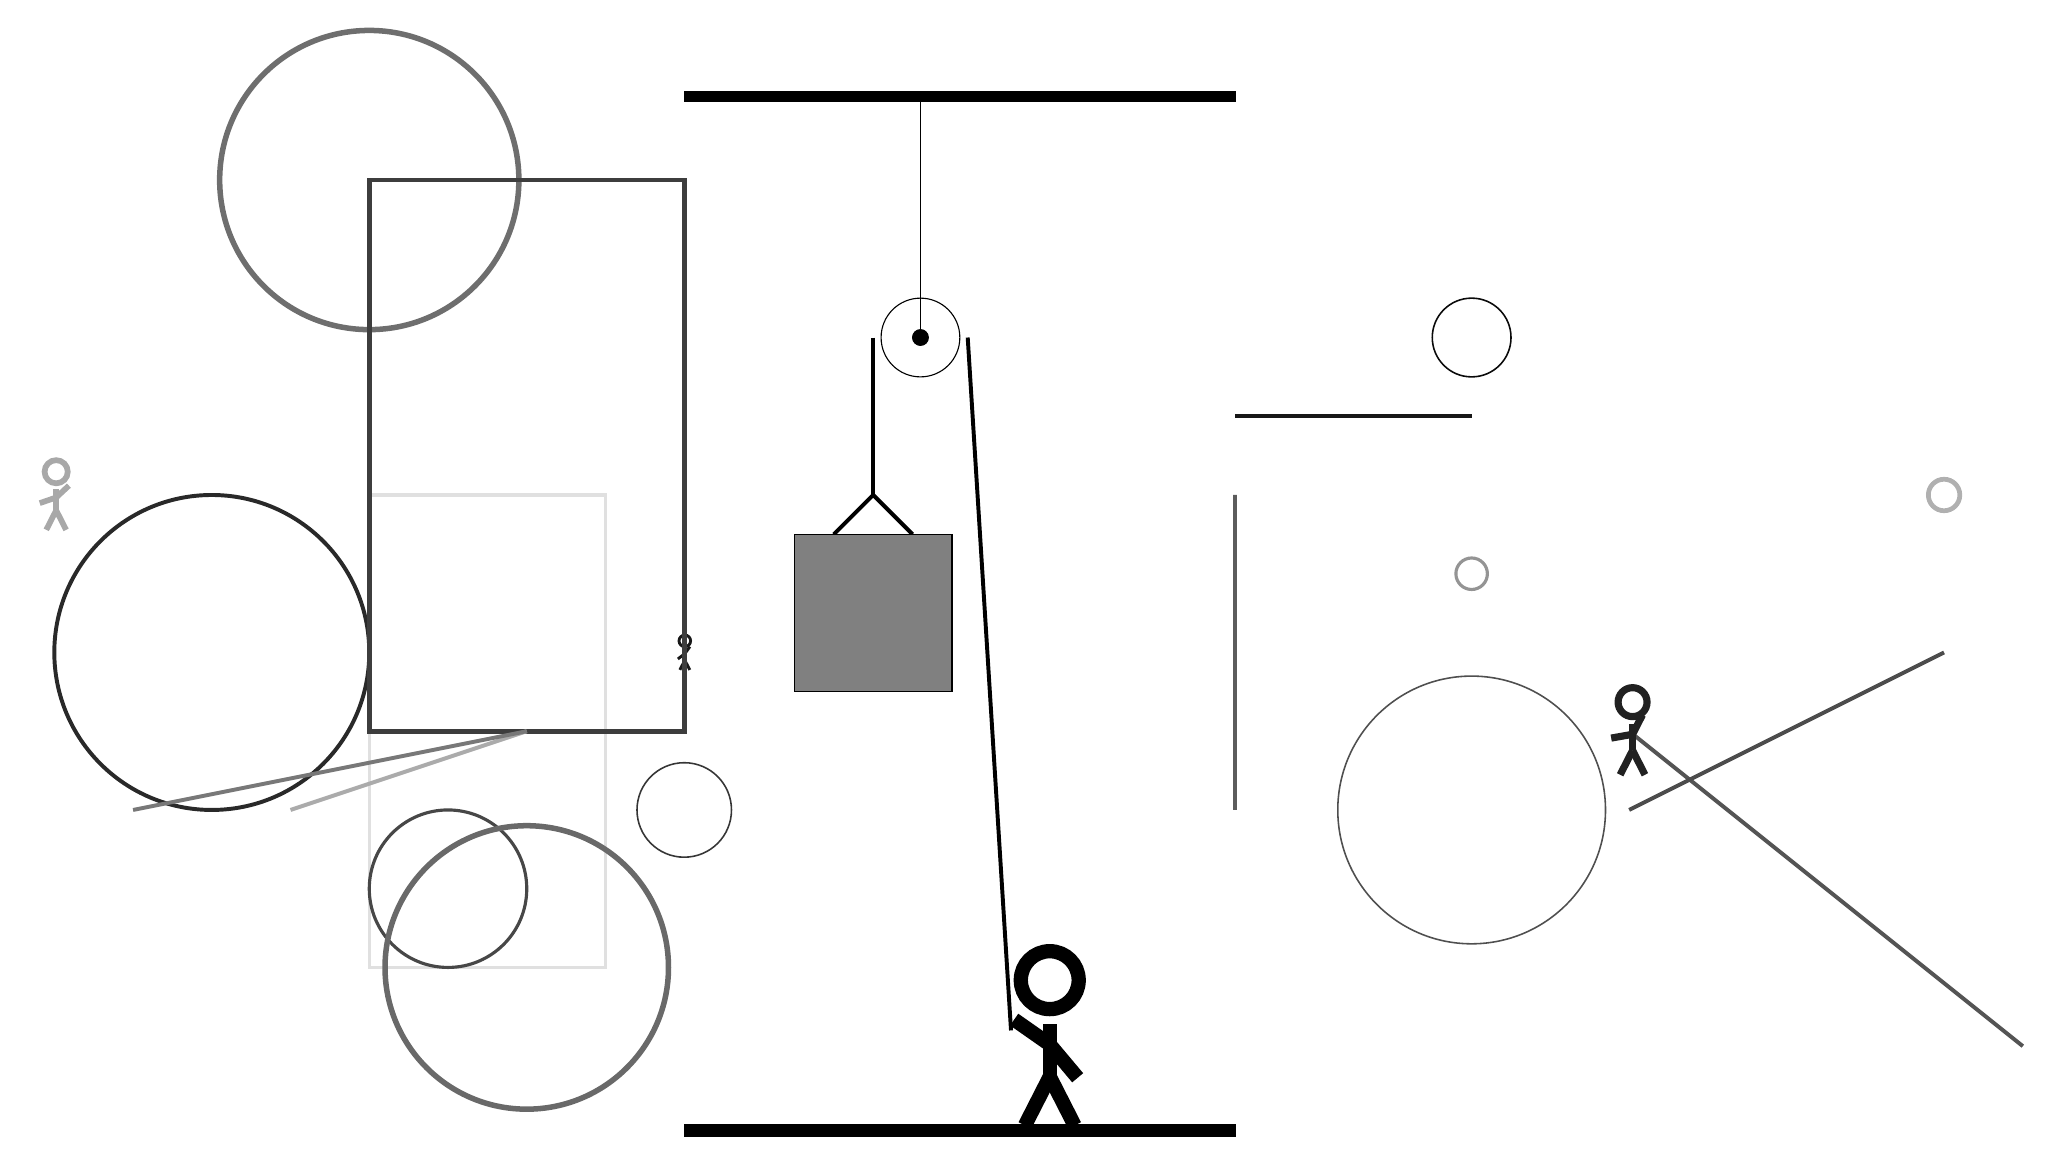
\begin{tikzpicture}
		%%%%% START %%%%%
		
		\draw[fill=black] (-2, 10) rectangle (5, 10.125);
		
		\draw (1, 7) circle (0.5);
		\draw[fill=black] (1, 7) circle (0.1);
		\draw (1, 10) -- (1, 7);
		
		\draw[line width=0.5mm] (-0.1, 4.5) -- (0.4, 5.0) -- (0.9, 4.5);
		\draw[fill=black!50] (-0.6, 4.5) rectangle (1.4, 2.5);
		
		\draw[line width=0.5mm] (0.4, 7) -- (0.4, 5.0);
		\centerarc[line width=0.5mm](1, 7)(0:180:0.6);
		\draw[line width=0.5mm](1.6, 7) -- (2.15, -1.8);
		
		\node at (2.6, -1.9) {\Strichmaxerl[10][-35][-50]};
		
		\draw [line width=0.2mm, color=black!96](8, 7) circle (0.5);
		
		\draw [line width=0.7mm, color=black!57](-6, 9) circle (1.9);
		\draw[line width=0.4mm, color=black!12] (-3, 5) rectangle (-6, -1);
		\node[line width=0.5mm, color=black!34] at (-10, 5) {\Strichmaxerl[4][19][43]};
		
		\draw[line width=0.5mm, color=black!67](10, 2) -- (15, -2);
		\draw [line width=0.4mm, color=black!72](-5, 0) circle (1.0);
		
		\node[line width=0.6mm, color=black!91] at (-2, 3) {\Strichmaxerl[2][37][54]};
		\draw [line width=0.2mm, color=black!79](-2, 1) circle (0.6);
		\draw [line width=0.5mm, color=black!84](-8, 3) circle (2.0);
		\draw [line width=0.7mm, color=black!59](-4, -1) circle (1.8);
		\node[line width=0.2mm, color=black!87] at (10, 2) {\Strichmaxerl[5][10][63]};
		\draw[line width=0.5mm, color=black!70](10, 1) -- (14, 3);
		\draw [line width=0.4mm, color=black!42](8, 4) circle (0.2);
		
		\draw[line width=0.6mm, color=black!76] (-2, 9) rectangle (-6, 2);
		\draw [line width=0.2mm, color=black!69](8, 1) circle (1.7);
		\draw[line width=0.5mm, color=black!64] (5, 5) rectangle (5, 1);
		
		\draw[line width=0.5mm, color=black!91](8, 6) -- (5, 6);
		
		\draw[line width=0.5mm, color=black!33](-7, 1) -- (-4, 2);
		\draw[line width=0.5mm, color=black!53](-4, 2) -- (-9, 1);
		\draw [line width=0.6mm, color=black!31](14, 5) circle (0.2);
		
		\draw[fill=black] (-2, -3) rectangle (5, -3.15);
		
		%%%%% END %%%%%
	\end{tikzpicture}
\end{document}